% Requirements to address here:
%
% Develop an agile, fit-for-purpose and sustainable service offering
% accessible through the EOSC hub that can satisfy the evolving needs of
% the scientific community by stimulating the design and prototyping of
% novel innovative digital services. Innovative models of collaboration
% that genuinely include incentive mechanisms for a user oriented open
% science approach should be considered.

\subsection{Relation to the Work Programme}

The \TheProject project addresses the challenges of the ``Prototyping
new innovative services'' call (ID: INFRAEOSC-02-2019).

Our strategy is based on taking the increasingly popular Jupyter
Notebook and the Jupyter Ecosystem: we want to evolve and improve them
so that others can build new innovative services based of the Jupyter
tools for the EOSC.
\medskip

There is evidence that the Jupyter Notebook is an e-infrastructure
that is useful across many domains: is is already widely adopted in
numerous communities and used by millions of researchers worldwide
\cite{jupyter-grant}.

\begin{itemize}
\item \emph{Journalists} and practitioners of \emph{data-driven
    journalism} at the LA Times, BuzzFeed News, Columbia Journalism School \cite{latimes-datadesk} \cite{columbia-nytimes} \cite{data-journalism},
\item \emph{Research institutions} such as CERN, JRC, and many more,
  operating institution-wide Jupyter deployment,
\item \emph{Universities} using Jupyter as a teaching platform,
\item \emph{Large cloud providers} building commercial products on the
  top of Jupyter (Google DataLab, Amazon Sagemaker, Microsoft Azure
  Notebooks),
\item \emph{Other EOSC projects}. Jupyter is already planned to become
  an important service on the European Open Science Cloud (for example
  the EOSC-04-funded PaNOSC project \cite{panosc}).
\item \emph{Data scientists}: some argue that the Jupyter Notebook is
  \emph{the} tool of choice for data scientists across domains
  \cite{Perkel2018}.
\item Over 3 million notebooks are deposited on GitHub \cite{notebookcount}.
\end{itemize}
%
\begin{figure}[tb]
  \centering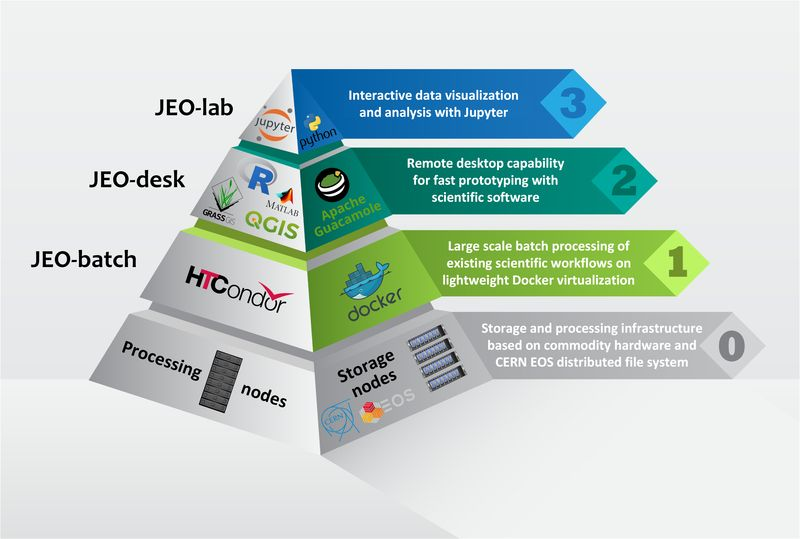
\includegraphics[height=0.2\textheight]{images/jeodpp.png}
  \centering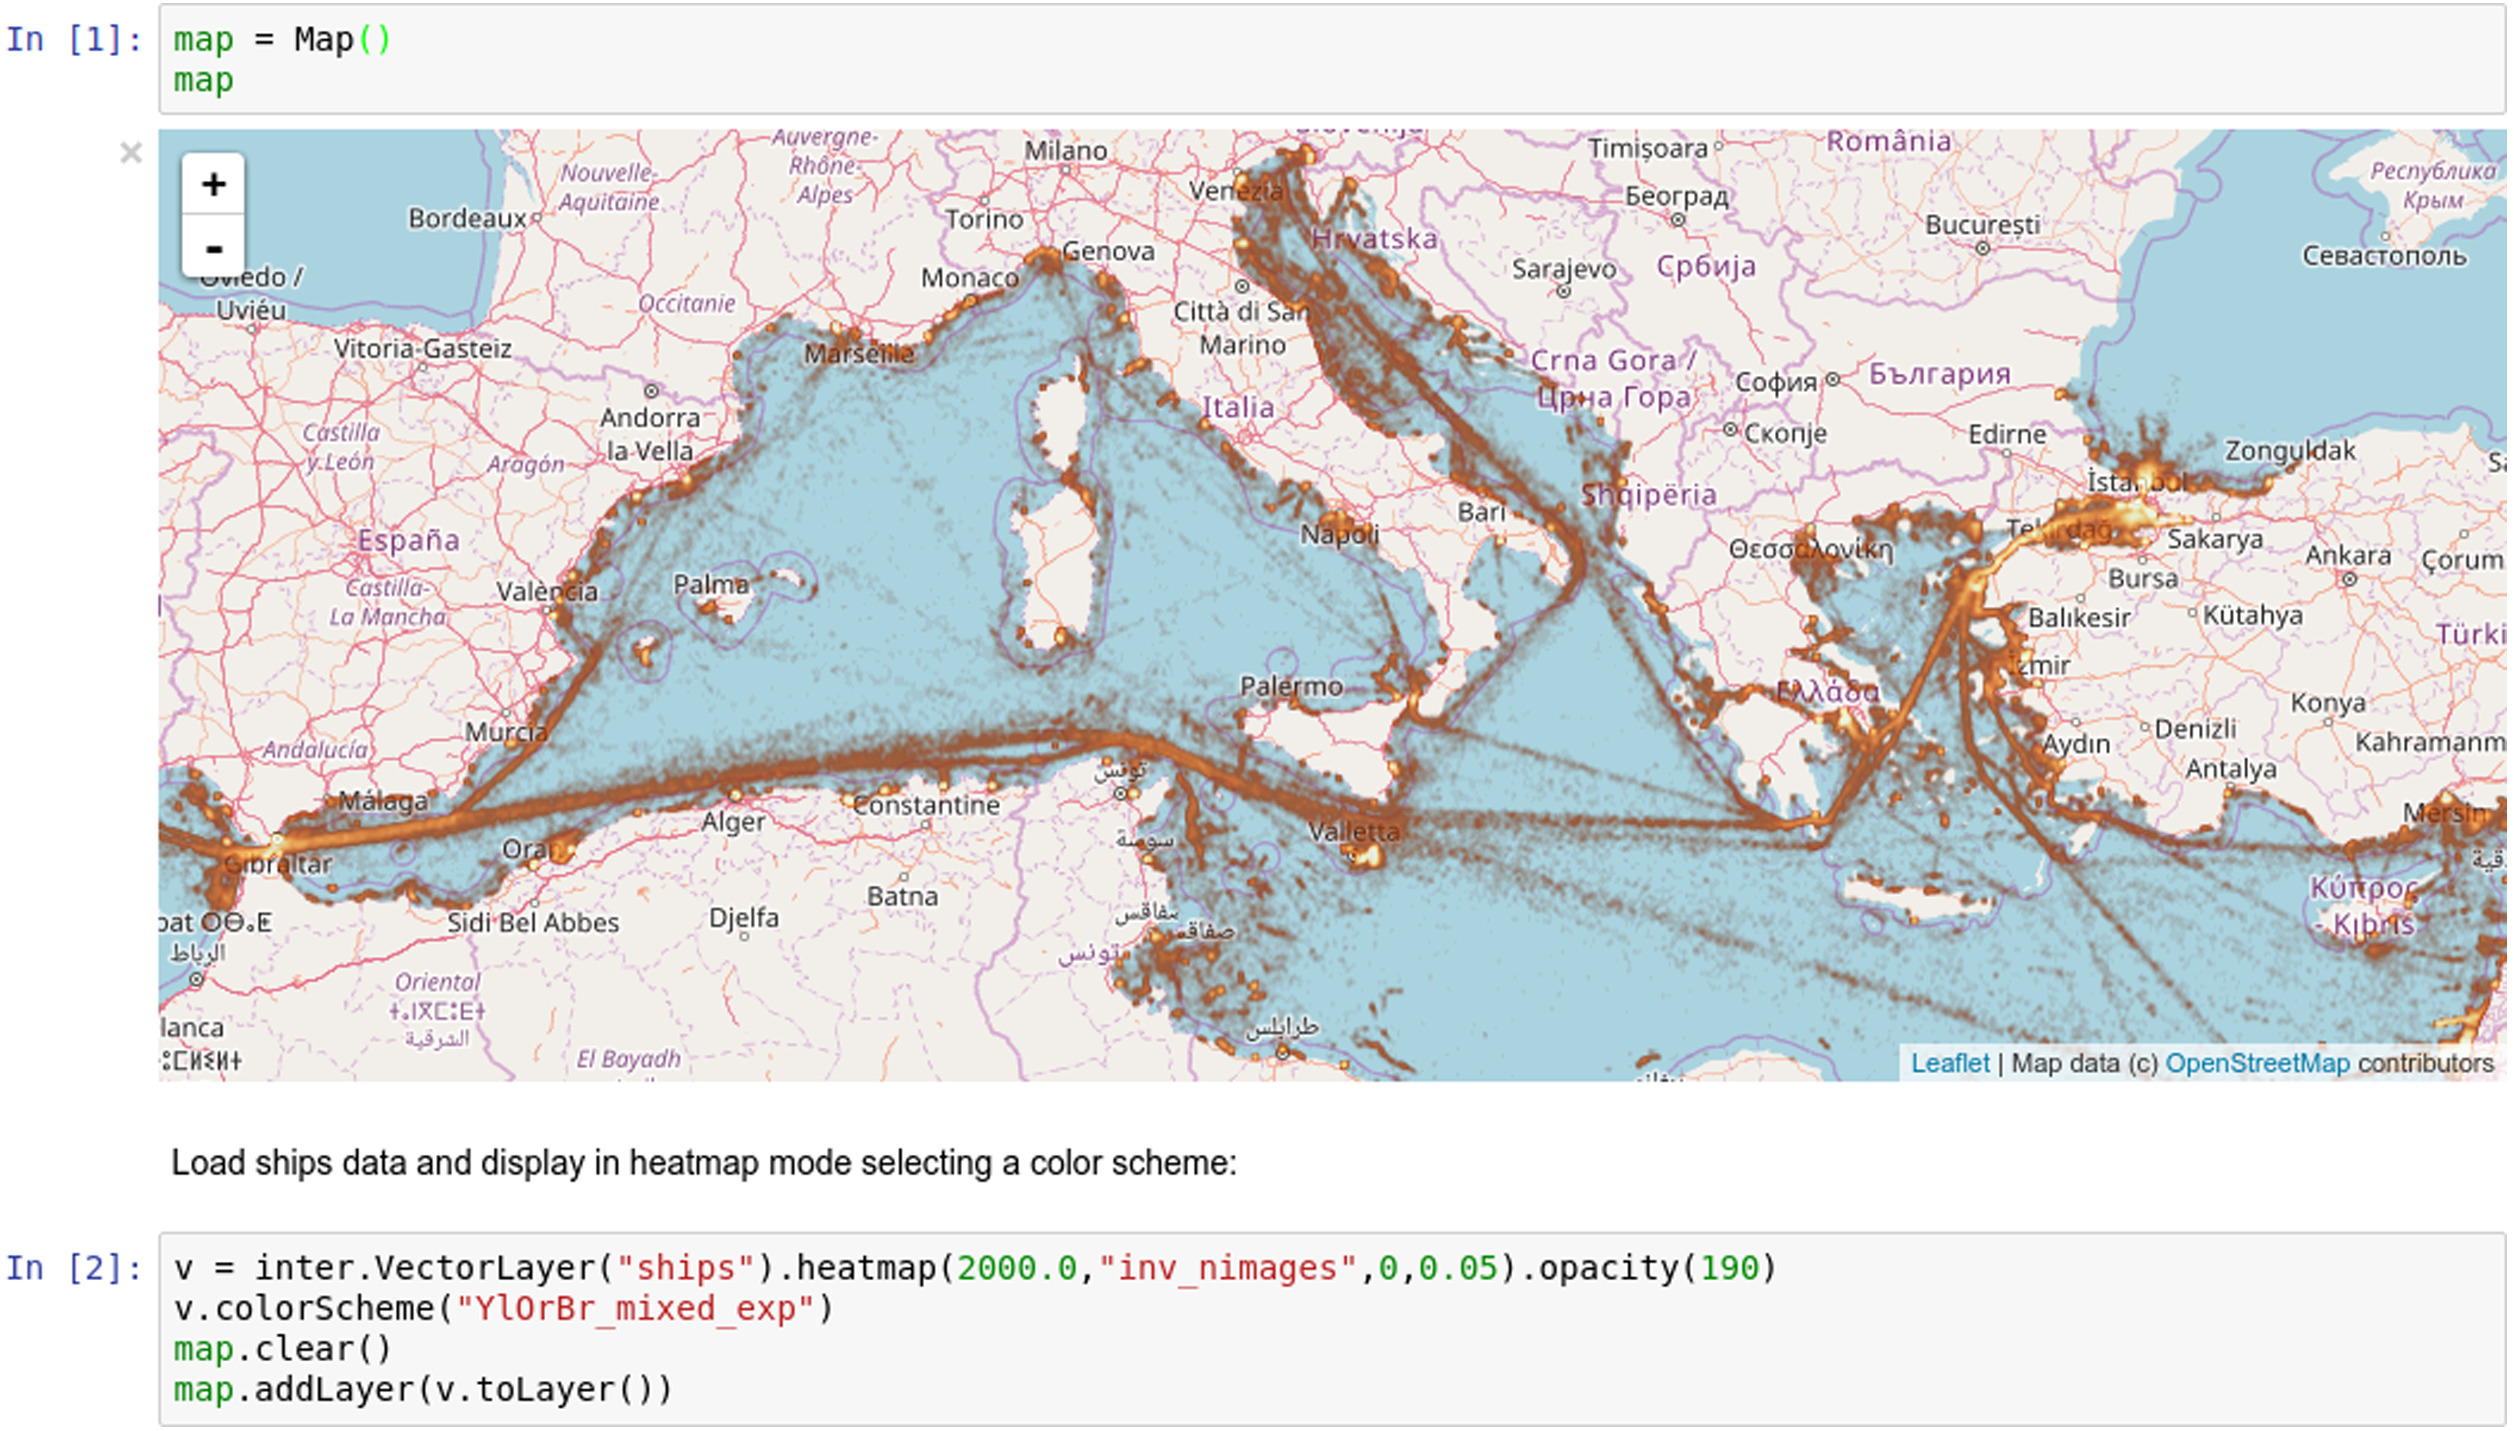
\includegraphics[height=0.2\textheight]{images/jeodpp-demo.jpg}
  \caption{\emph{Left}: The Joint Research Centre (JRC) Earth Observation
    Data and Processing Platform (JEODPP) is a heavy user of the
    Jupyter Notebook (source:
    \url{https://cidportal.jrc.ec.europa.eu/home/}), where it features
    at the top of the pyramid to help users with interactive data
    visualisation and analysis. \emph{Right}: An example
    service in which an interactive visualisation is provided through
    the Jupyter notebook rendering of the density map of the ships
    detected from Sentinel-1 images over the Mediterranean sea during
    the period October 2014 to September 2016. \cite[Figure
    6]{Soille2018}. \label{fig:jeodpp}}
\end{figure}
%
A particular example is the Joint Research Centre Earth Observation
Data and Processing Platform (JEODPP) shown in Fig.~\ref{fig:jeodpp},
illustrating the interactive data exploration within an environment
that allows to save and communicate the data exploration
conveniently. These projects are building upon Jupyter as it is
available at the moment.
\bigskip

Within this context of a common software platform, we address the call
for prototyping innovative services:
\begin{itemize}
\item Our \TheProject proposal is focussed on developing the next generation
of the Jupyter tools to enable all domains to develop such services on
the EOSC.

\item Through the \TheProject-improved Jupyter, we will provide an
  agile and fit-for-purpose \emph{EOSC-enabled
framework} within which innovative services can be build by the
scientific communities.

\item We believe this is realistic as a multitude of (non-EOSC) services and
  use cases based on Jupyter have been developed, as sketched above.

\item We will provide some particular services as part of the project
  (in the domains of astronomy, geosciences, health, mathematics, education and photon
  science) to stimulate the design of other novel innovative services
  to address the evolving needs of the scientific community.

\item We co-design the framework and the service demonstrators with
  core Jupyter developers, EGI and domain specialists from the
  scientific communities
\end{itemize}
\bigskip


%
% % [1] EINFRAOESC-02 call (\url{https://ec.europa.eu/info/funding-tenders/opportunities/portal/screen/opportunities/topic-details/infraeosc-02-2019;freeTextSearchKeyword=innovative;typeCodes=0,1;statusCodes=31094501,31094502;programCode=null;programDivisionCode=null;focusAreaCode=null;crossCuttingPriorityCode=null;callCode=Default;sortQuery=openingDate;orderBy=asc;onlyTenders=false)}
%
% Jupyter is an important piece of infrastructure for numerous projects funded
% by the EU and its member states, including OpenDreamKit, PaNOSC, EOSC-life,
% JEODPP \cite{Soille2018}, \TODO{citations? others?}... The \TheProject project
% will thus act like a catalyst, increasing the potential impact of all these
% projects, as well as hopefully many future projects, by strengthening a common
% software platform.
%
%
%
% % Lots of EOSC and EU-funded projects are built upon jupyter
% %
% % Opendreamkit
% % PaNOSC
% % JEODPP https://www.sciencedirect.com/science/article/pii/S0167739X1730078X?via%3Dihub
% % EOSC-Pilot
% % EGI https://ec.europa.eu/info/funding-tenders/opportunities/portal/screen/opportunities/topic-details/infraeosc-02-2019;freeTextSearchKeyword=innovative;typeCodes=0,1;statusCodes=31094501,31094502;programCode=null;programDivisionCode=null;focusAreaCode=null;crossCuttingPriorityCode=null;callCode=Default;sortQuery=openingDate;orderBy=asc;onlyTenders=false
% %
% % Jupyter is a critical piece of European e-infrastructure; this project is important for sustainability, we need not just to build upon Jupyter but to consolidate the foundations.
% %
% % We also want to enable novel use cases to enable advances in European computational and data science activities that build on the Jupyter ecosystem.
% %
% % Who is better placed than the team who built Jupyter in the first place to move Jupyter forward?
% %
% % JEODPP Image (jeodpp_new_small_4.png)
% %
% %
% % The main challenge we need to address is “Develop an agile, fit-for-purpose and sustainable service offering accessible through the EOSC hub that can satisfy the evolving needs of the scientific community by stimulating the design and prototyping of novel innovative digital services. Innovative models of collaboration that genuinely include incentive mechanisms for a user oriented open science approach should be considered.” (from Specific challenge in: https://ec.europa.eu/info/funding-tenders/opportunities/portal/screen/opportunities/topic-details/infraeosc-02-2019;freeTextSearchKeyword=innovative;typeCodes=0,1;statusCodes=31094501,31094502;programCode=null;programDivisionCode=null;focusAreaCode=null;crossCuttingPriorityCode=null;callCode=Default;sortQuery=openingDate;orderBy=asc;onlyTenders=false)
% %
% % We need to make sure to either put this phrase in and respond to how we address it, or drop the right keywords.
% %
% %
% % \TODO{We should also go through the requirements from the call [1] and
% %   show how we address those [to provide easily accessible evidence
% %   that we are addressing the call].}
% %
